
La dernière alerte modélisée est le cas dit du \enquote{fil rouge} que
nous avions présenté dans le premier chapitre de cette thèse. Comme
nous l'avions indiqué lors de sa première présentation, le \emph{fil
  rouge} est une alerte particulière, contenant de nombreux indices
très imprécis et incertains. Par conséquent la \ac{zir} est
extrêmement étendue.


\subsection{Présentation de l'alerte}
\label{subsec:9-4-1}

Le fil rouge est une alerte composée de XX \emph{indices de
  localisation.}


Faute d'enregistrement audio, le fil rouge n'a pas été retranscrit,
les indices dont nous disposons (et qui avaient été présentés dans le
\autoref{chap:01}) ont donc été directement saisis par le secouriste.
%
de ce fait, le \emph{fil rouge} est une alerte assez différente des
précédentes, puisque XXX n'est pas
%
Le traitement du \emph{fil rouge} est donc plus proche du traitement
opérationnel qui sera réellement effectué lors du traitement d'une
alerte.


Pour le cas du \emph{fil rouge} nous ne disposons pas de
l'enregistrement audio et donc de son verbatim, les indices ayant déjà 
été synthétisés par les secouristes. Les les avions déjà présentés
dans le \autoref{chap:01}.
%
Pour rappel voici la synthèse de l'alerte qui nous a été donnée par
les secouristes :
%
\begin{enumerate}
\item La victime est partie de Bourg d'Oisans, à pied, sur chemin, en
  direction d'une station de ski.
\item La victime a marché plusieurs heures.
\item La victime a chuté de plusieurs mètres.
\item La victime voit une partie de plan d'eau.
\item La victime est sous une route et entend des véhicules.
\item La victime est sous une ligne électrique 3 brins.
\item La victime vient de passer du soleil à l'ombre.
\end{enumerate}


Comme on peut le remarquer, ces indications 

La première description nous donne de nombreuses informations, 

La seconde description nous indique que la victime a marché plusieurs
heures. Ici le point de départ et la direction ne sont pas
explicitement mentionnés.

Le troisième élément donné par le secouriste indique que la victime
a chuté

Vient ensuite la quatrième description



XXXXXXXXXXX
% 
\begin{enumerate}
\item \label{ind:fr1} La victime est en direction de
  % 
\item \label{ind:fr2} La victime est
  \onto[orl]{A\-Temps\-De\-Marche\-De} \emph{Bourg-d'Oisans} 
  % 
\item \label{ind:fr3} La victime est \onto[orl]{Sous\-Proche\-De} un
  chemin
  % 
\item \label{ind:fr4} La victime voit
  % 
\item \label{ind:fr5} La victime est \onto[orl]{Sous\-Proche\-De} une
  route
  % 
\item \label{ind:fr6} La victime est \onto[orl]{Sous\-Proche\-De} une
  ligne électrique trois brins
\end{enumerate}



\subsection{Modélisation de l'alerte}
\label{subsec:9-4-2}

La \ac{zir} définie pour cette alerte est une zone de
\SI{625}{\kilo\meter\squared}

\begin{figure}
  \centering
  \begin{tikzpicture}
  \tikzset{et/.style={above,font=\footnotesize\vphantom{Ag}}}
  % 
  \node[inner sep=0pt, anchor=south west] (image) at (0,0){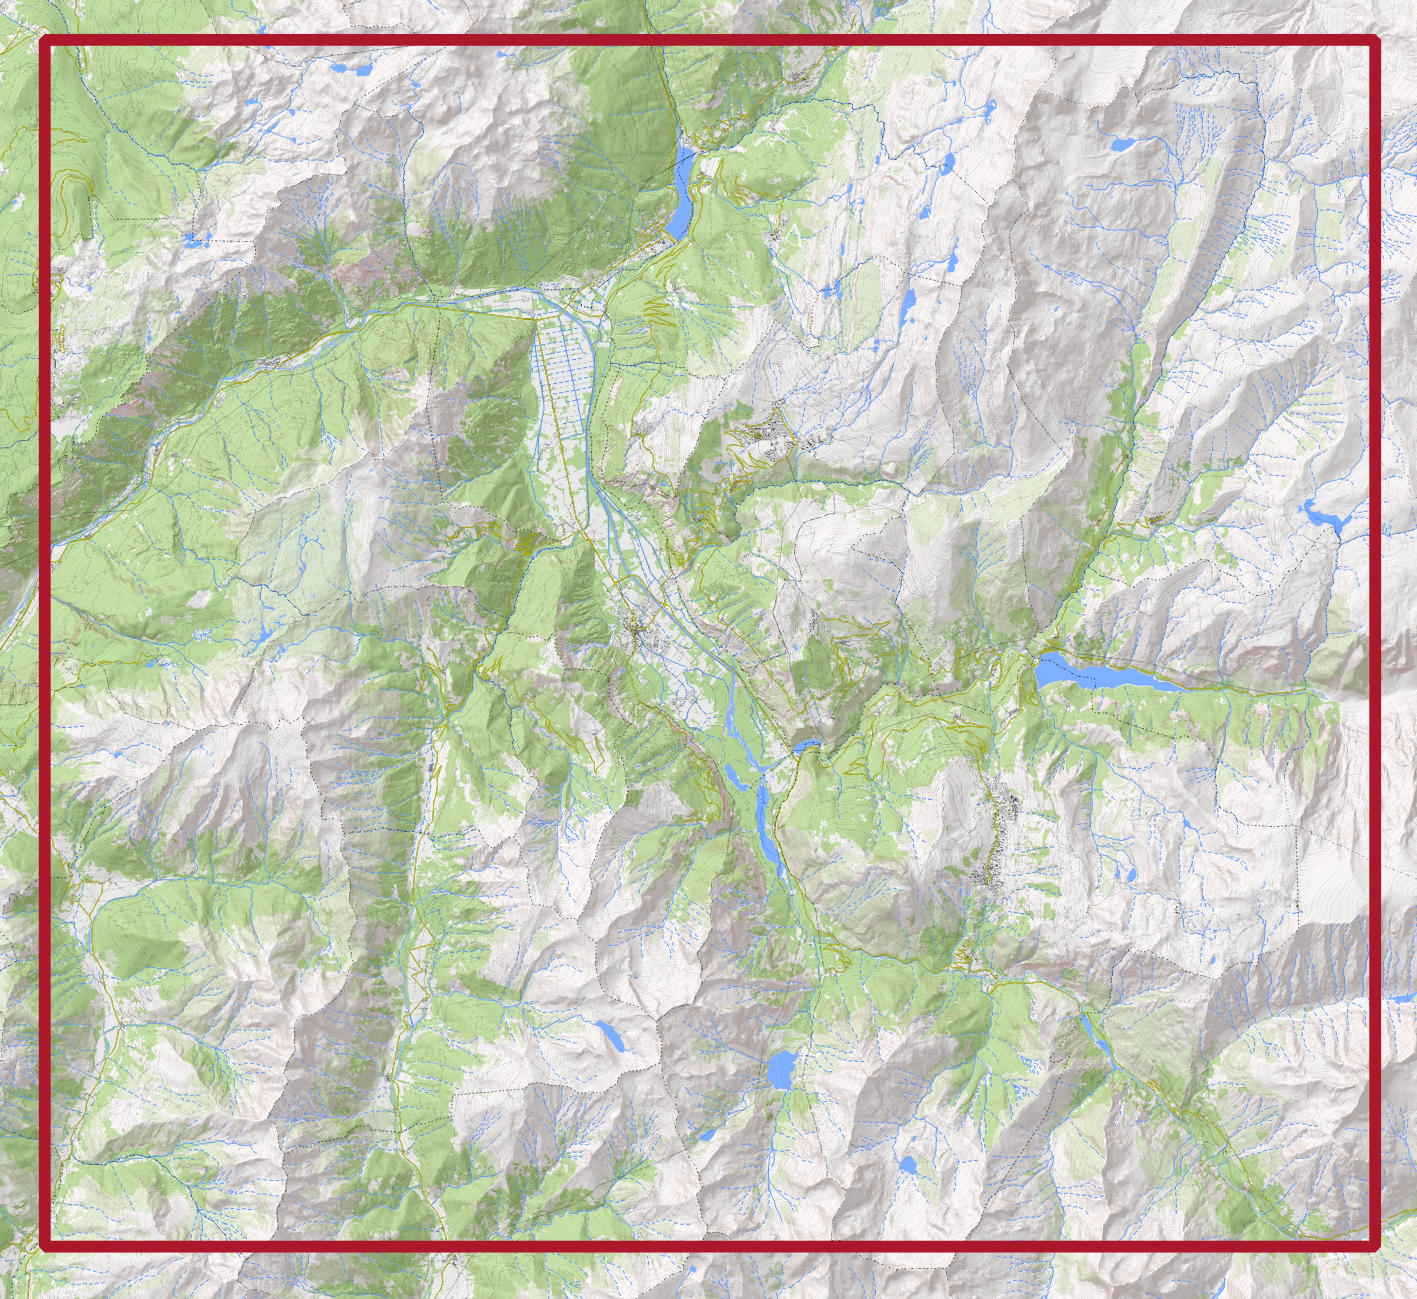
\includegraphics{./figures/ZIR_fil_rouge.png}};
  % 
  \begin{scope}
    \node (P2) at ([yshift=-.5cm]image.south east) {};
    \node (P1) at ([yshift=-.5cm]image.south west) {};
    % 
    \node (rect) [anchor=north west, minimum width=1cm,minimum
    height=.25cm] at ([yshift=-.25cm]P1) {}; \path[draw=RdBu-9-1, line
    width=1mm](rect.west) --([xshift=-1ex]rect.south) -- ([xshift=1ex]rect.north)
    -- (rect.east);
    % 
    \node[anchor=west, font=\tiny\vphantom{Ag}, text width = 4cm] at
    ([xshift=1ex]rect.east) {Limite de la \ac{zir}};
    % Échelle
    % Échelle
    \draw[-] (P2 |- -1cm,-1cm) --++ (-1,0) node[et,pos=.5] {\SI{2}{\kilo\meter}};
    % Légende détaillée
    \path (P1) -- (P2) node[pos=.5, yshift=-1cm] {\tiny Pour la légende détaillée du fond topographique voir \autoref{anx:topo_leg}. Sources: BD TOPO 2018, BD ALTI 2018.}; 
  \end{scope}
\end{tikzpicture}
  \caption{Zone initiale de recherche pour le \emph{fil rouge}}
  \label{fig:zir_fil_rouge}
\end{figure}

\subsubsection{Décomposition des indices de localisation}
\label{subsec:9-4-2-1}

\subsubsection{Spatialisation des indices de localisation}
\label{subsec:9-4-2-2}

\subsubsection{Fusion des zones de localisation compatibles}
\label{subsec:9-4-2-3}

\subsection{Critique de la modélisation}
\label{subsec:9-4-3}

%%% Local Variables:
%%% mode: latex
%%% TeX-master: "../../../../main"
%%% End:
